%----------------------------------------------------------------------------
\chapter{\bevezetes}
%----------------------------------------------------------------------------


The digital era has led to large amounts of data being amassed by companies every day. Data comes from multiple sources: sensors, sales data, communication systems, logging of system events \etc. According to Forbes \cite{Forbes} 2.5 quintillion bytes of data created each day. That means 2.5 million Terabytes per day. Bigger corporations can easily create hundreds of Terabytes a day. So we need a new solution to process this amount of data. The traditional relational databases (RDBMS) can deal only with Gigabytes. Hadoop provides a software framework to scale up our system for storing, processing and analyzing big data.

In this chapter, I will write about the basics of Hadoop architecture, why Hive was created on top if it and the performance issues it faces.

\section{Hadoop basics}
Apache Hadoop is an open source distributed framework for managing, processing  and storing a huge amount of data in clustered systems built from commodity hardware. All modules in Hadoop was designed with an assumption that hardware failures are common and should be automatically handled by the framework. One of the most important characteristic of Hadoop that it partitions the data and computation across many hosts and executing computation in parallel close to the data it uses.  \cite{Hadoop-wiki}

The base of the Hadoop framework contains the following modules:
\begin{itemize}
	\item HDFS - Hadoop Distributed File System: designed to store large data sets reliably and stream those at high bandwidth to user applications.
	\item Hadoop MapReduce: an implementation of the MapReduce programming model for large data processing
	\item YARN - Yet Another Resource Negotiator: a resource management and job scheduling technology
	\item Hadoop Common: contains libraries and utilities needed by other Hadoop modules
\end{itemize}
\subsection{Hadoop \vs traditional databases}
Traditional databases cannot be used when we want to process and store big data. The main differences between Hadoop and traditional RDBMS:
\begin{itemize}
	\item \textbf{Data Volume}: RDBMS works better when the data volume is low (Gigabytes). However when data size is huge (Terabytes-Petabytes) traditional databases fail. On the other hand Hadoop can easily handle this amount of data.
	\item \textbf{Data Variety}: this generally means the type of data to be processed. Hadoop has the ability to store and process data whether it is structured, semi-structured or unstructured. Even though  it is mostly used for large amount of unstructured data. 
	In contrast, traditional RDBMS can only be used to manage structured or semi-structured data. 
	\item \textbf{Scalability}: RDBMS provides vertical scalability. You can add more resources, memory or CPU to a machine in the cluster. Whereas Hadoop provides horizontal scalability. It means we can add more machines to an existing cluster. As a result of this Hadoop becomes fault tolerant. We can easily recover data in case of a failure of one of the machines.
	\item \textbf{Data Processing}: Apache Hadoop supports OLAP (Online Analytical Processing) that involves very complex queries and aggregations. The database design is de-normalized, having fewer tables. On the other hand, RDBMS supports OLTP (Online Transaction Processing), which involves fast query processing. The database design is normalized having large number of tables. \cite{Hadoop-vs-RDBMS}
\end{itemize}
\subsection{HDFS - Hadoop Distributed File System}
HDFS is the file system of Hadoop. It stores file system metadata and application data separately. The dedicated server that stores metadata is the NameNode. Application data are stored on other servers (DataNodes). These servers are connected and they communicate using TCP-based protocols. 
\subsubsection*{NameNode \cite{Secondary-NameNode}}
NameNode keeps the directory tree of all files in the file system and tracks where file data is kept across the cluster. It does not store the files itself. Clients talk to the NameNode whenever they want to locate or add/move/copy/delete a file. The NameNode returns a list of relevant DataNode servers where the data is available. 

As a result of this approach, the NameNode is a Single Point of Failure in the HDFS cluster. Whenever the NameNode goes down, the file system becomes offline.
\begin{figure}[H]
	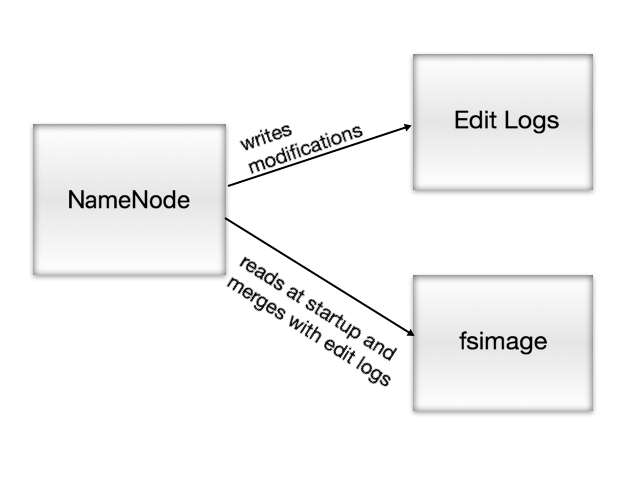
\includegraphics[width=80mm, keepaspectratio]{figures/namenode_problem.png}
	\centering
	\caption*{Problem with the NameNode}
\end{figure}
The image shows how NameNode stores information. There are two different files:
\begin{itemize}
	\item edit logs: the changes made to the file system after the NameNode started
	\item fsimage: a snapshot of the file system when the NameNode started
\end{itemize}
In production clusters the NameNode restarts are very rare that means edit logs can grow large therefore in case of a crash we will lose huge amount of metadata since the fsimage is very old.

The Secondary NameNode helps to address this issue. It takes over the responsibility of merging the edit logs with fsimage. It collects edit logs on a regular basis and applies them to the fsimage. NameNode will use this fsimage in case of a crash and it can also be used to reduce the startup time of the NameNode since it can use the fsimage for next restart.
It is important to remember that the Secondary NameNode is not a real backup NameNode it only merges the edits into the fsimage. 

\begin{figure}[H]
	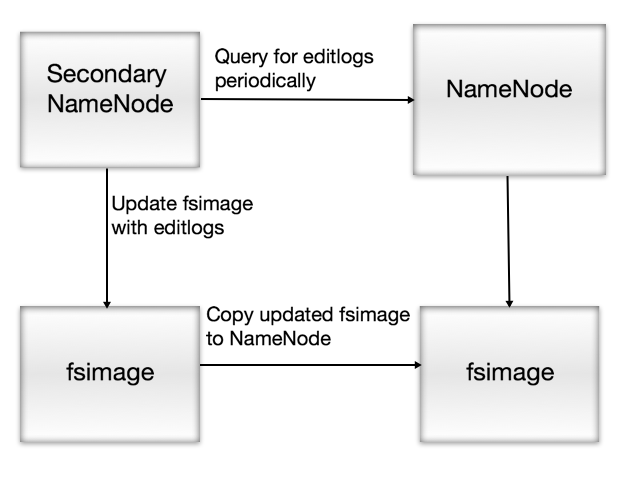
\includegraphics[width=80mm, keepaspectratio]{figures/secondary_namenode.png}
	\centering
	\caption*{Solution using the Secondary NameNode}
\end{figure}

\subsubsection*{DataNodes}
On a DataNode a block is represented by two files on the host's native file system. The first contains the data itself, the second is the metadata: checksum for the data and generation stamp. 

On startup, the DataNodes connect to the NameNode and perform a handshake. The reason for the handshake, is to verify the namespace ID and software version of the DataNodes. If one of them does not match with the NameNode's value, the DataNode automatically shuts down. After a successful handshake the DataNode registers with the NameNode. DataNode will store it's internal identifier persistently. This way, if restart occurs the DataNodes will be recognizable even if they get a different IP address or port. After the ID is registered to the NameNode the ID of a DataNode will never change. 

 When a DataNode is registered it sends a block report immediately. It contains  block id, generation stamp and the length of each block the DataNode server hosts. To provide up-to-date information to the NameNode reports are sent every hour. 

During normal operation, DataNodes send heartbeats to the NameNode. It ensures the NameNode that the DataNode is operating and block replicas of the server are available. If the NameNode does not receive a heartbeat from a DataNode it will consider the node to be out of service. The default heartbeat interval is three seconds.

\subsubsection*{HDFS Client}
User applications access the file system using the HDFS client. It exports the HDFS file system interface. Similar to a traditional file system, HDFS supports operations to read, write and delete files and to create or delete directories. The user references files and directories by paths in the namespace. 

When someone reads a file, HDFS Client asks the NameNode for the list of DataNodes that host replicas of the blocks of the file. Then it will directly contacts the DataNode and request the desired block. When the client writes, it asks the NameNode to choose DataNodes to host replicas of the first block of the file. When the first block is filled, the client requests for new DataNodes to place the next blocks.

\begin{figure}[H]
	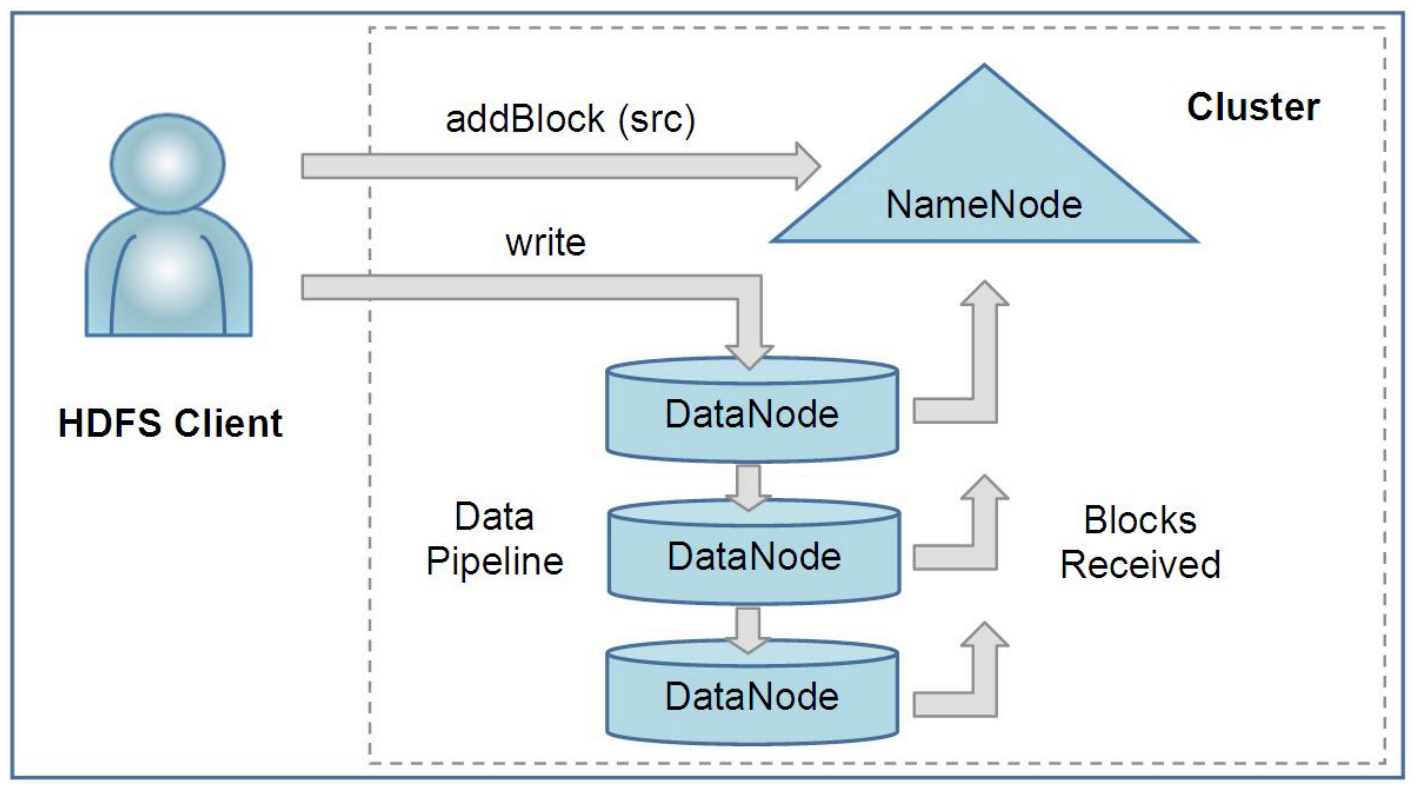
\includegraphics[width=100mm, keepaspectratio]{figures/hdfs_client.png}
	\centering
\end{figure}
The client creates a new file by giving its path to the NameNode. For each block, the NameNode will return a list of DataNodes to place the replicas. The client pipelines data to the given DataNodes, and they will confirm the creation of the block to the NameNode
\subsection{MapReduce}
\subsection{Yarn}